\section{分组密码:基本定义与性质}\label{sec:4-1}

从功能上讲,\textbf{分组密码}是一种确定性密码 $\mathcal{E}=(E,D)$,其消息空间和密码空间是同一(有限)集 $\mathcal{X}$。如果 $\mathcal{E}$ 的密钥空间是 $\mathcal{K}$,我们就称 $\mathcal{E}$ 是一个\textbf{定义在 $(\mathcal{K},\mathcal{X})$ 上}的分组密码。我们称元素 $x\in\mathcal{X}$ 为一个\textbf{数据分组(data block)},并称 $\mathcal{X}$ 为 $\mathcal{E}$ 的\textbf{数据分组空间}。

对于每个固定的密钥 $k\in\mathcal{K}$,我们可以定义函数 $f_k:=E(k,\cdot)$;也就是说,$f_k:\mathcal{X}\to\mathcal{X}$ 可以把 $x\in\mathcal{X}$ 映射为 $E(k,x)\in\mathcal{X}$。密码的正确性属性要求,对于任意的固定密钥 $k$,函数 $f_k$ 都是一一对应的,并且由于 $\mathcal{X}$ 是有限集,$f_k$ 也必须在有限集上。因此,$f_k$ 本质上就是有限集 $\mathcal{X}$ 上的一个置换,而 $D(k,\cdot)$ 是其逆置换 $f^{-1}_k$。

尽管从语法上讲,分组密码只是一种特殊的密码,但我们期望分组密码具备比语义安全性强得多的安全属性:对于一个随机选择的密钥 $k$,就所有的实际情况而言,置换 $E(k,\cdot)$ 都应该``看起来"像一个随机置换。我们下面会更精确地定义这一概念。

一个非常重要且流行的分组密码是高级加密标准 (Advanced Encryption Standard, AES)。我们将在后面详细地研究 AES 的内部设计,但现在我们先给出一个非常顶层的描述。AES 的密钥通常是 $128$ 比特的序列(但也可以使用更长的密钥,比如 $192$ 比特或 $256$ 比特)。AES 数据分组是 $128$ 比特的序列,见图 \ref{fig:4-1}。AES 的设计是相当高效的:使用一台典型的消费级计算机进行一次 AES 加(解)密仅需几百个时钟周期。

\begin{figure}
  \centering
  \tikzset{every picture/.style={line width=0.75pt}}      

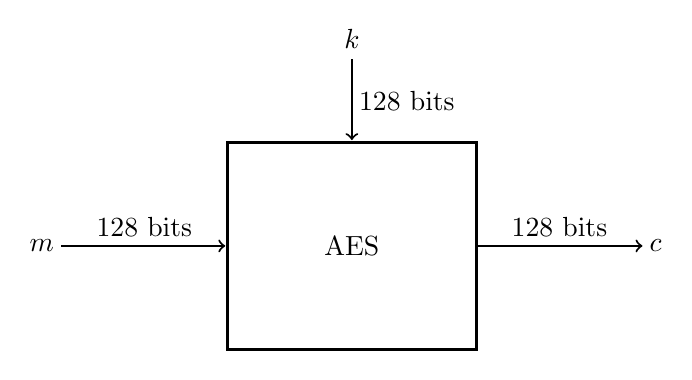
\begin{tikzpicture}[x=0.75pt,y=0.75pt,yscale=-1,xscale=1]

\draw  [line width=1.2]  (100,60) -- (220,60) -- (220,160) -- (100,160) -- cycle ;

\draw  [->]  (20,110) -- (99,110) ;
\draw  [->]  (220,110) -- (300,110) ;
\draw  [->]  (160,20) -- (160,59) ;

\draw (160,110) node   [align=left] {AES};
\draw (60,107) node [anchor=south] [inner sep=0.75pt]   [align=left] {$ 128$ bits};
\draw (260,107) node [anchor=south] [inner sep=0.75pt]   [align=left] {$ 128$ bits};
\draw (162,40) node [anchor=west] [inner sep=0.75pt]   [align=left] {$ 128$ bits};
\draw (18,110) node [anchor=east] [inner sep=0.75pt]    {$m$};
\draw (302,110) node [anchor=west] [inner sep=0.75pt]    {$c$};
\draw (160,16.6) node [anchor=south] [inner sep=0.75pt]    {$k$};


\end{tikzpicture}
  \caption{分组密码 AES}
  \label{fig:4-1}
\end{figure}

分组密码的安全性定义被表述为一种``黑盒测试"。大致思路是这样的:一个有效对手被赋予一个``黑盒",盒子里是 $\mathcal{X}$ 上的一个置换 $f$,它来自以下两个随机过程中的一个:
\begin{itemize}
	\item $f=E(k,\cdot)$,其中 $k$ 是一个随机选出的密钥,或者
	\item $f$ 是从 $\mathcal{X}$ 的\emph{所有}置换中随机均匀选出的一个真随机置换。
\end{itemize}
对手无法看到盒子的内部,但它可以用提问的方式来``探测"它:它可以给盒子一个值 $x\in\mathcal{X}$ 并得到一个 $y:=f(x)\in\mathcal{X}$。我们允许对手发起多次提问,而且我们允许它以任何它想要的方式选择问题;特别地,这些问题甚至可以以某种巧妙的方式依赖于盒子对之前的某个或某些问题的回答。安全性意味着,对手无论如何也无法得知盒子里的是哪种类型的函数——是随机密钥控制的分组密码,还是一个真的随机置换。换句话说,一个安全的分组密码应该与一个随机置换\textbf{在计算上不可区分}。

为了更正式地定义这一概念,我们首先引入一些表记符号。我们用:
\[
{\rm Perms}[\mathcal{X}]
\]
表示 $\mathcal{X}$ 上\emph{所有}置换的集合。需要注意,这是一个非常大的集合:
\[
\big\lvert
{\rm Perms}[\mathcal{X}]
\big\rvert
=|\mathcal{X}|!
\]
对于 AES 来说,$|\mathcal{X}|=2^{128}$,因此,置换的数量约为:
\[
\big\lvert
{\rm Perms}[\mathcal{X}]
\big\rvert
\approx 2^{2^{135}}
\]
而 $128$ 比特的 AES 密钥所定义置换的数量最多为 $2^{128}$。

和之前一样,为了定义安全性,我们引入一个攻击游戏。就如定义 PRG 的攻击游戏一样,这个攻击游戏也包含两个独立的实验。在这两个实验中,对手将遵循相同的协议,即它会向挑战者提交一连串的查询 $x_1,x_2,\dots$;挑战者则用 $f(x_i)$ 回应查询 $x_i$。在第一个实验中,$f=E(k,\cdot)$,其中 $k\in\mathcal{K}$ 是随机选出的一个元素;而在第二个实验中,$f$ 是从 ${\rm Perms}[\mathcal{X}]$ 中随机选出的一个置换。在每个实验中,挑战者都只能使用同一个 $f$ 来回应所有来自对手的查询。当对手决定终止对挑战者的查询时,它就会输出一个比特。

\begin{game}[分组密码]\label{game:4-1}
对于一个定义在 $(\mathcal{K},\mathcal{X})$ 上的给定分组密码 $(E,D)$ 和一个给定对手 $\mathcal{A}$,我们定义两个实验:实验 $0$ 和实验 $1$。对于 $b=0,1$,我们定义:

\noindent\textbf{实验 $b$:}
\begin{itemize}
	\item 挑战者按如下方式选择 $f\in{\rm Perms}[\mathcal{X}]$:
	
	\hspace*{26pt} 如果 $b=0$:随机选取 $k\overset{\rm R}\leftarrow\mathcal{K}$,令 $f\leftarrow E(k,\cdot)$;\\
	\hspace*{26pt} 如果 $b=1$:随机选取 $f\overset{\rm R}\leftarrow{\rm Perms}[\mathcal{X}]$。
	
	\item 对手向挑战者发起一系列查询。\\
	对于 $i=1,2,\dots$,第 $i$ 个查询是一个数据分组 $x_i\in\mathcal{X}$。\\
	挑战者计算 $y_i\leftarrow f(x_i)\in\mathcal{X}$,并将 $y_i$ 交给对手。
	\item 对手计算并输出一个比特 $\hat b\in\{0,1\}$。
\end{itemize}

对于 $b=0,1$,令 $W_b$ 为 $\mathcal{A}$ 在实验 $b$ 中输出 $1$ 的事件。我们将 $\mathcal{A}$ 就 $\mathcal{E}$ 的\textbf{优势}定义为:
\[
\mathrm{BC}\mathsf{adv}[\mathcal{A},\mathcal{E}]
:=
\big\lvert
\Pr[W_0]-\Pr[W_1]
\big\rvert
\]
最后,如果 $\mathcal{A}$ 最多发起 $Q$ 次查询,我们就称 $\mathcal{A}$ 就是一个 \textbf{$Q$ 次查询 BC 对手}。
\end{game}

图 \ref{fig:4-2} 展示了攻击游戏 \ref{game:4-1} 中的两个实验。

\begin{definition}[安全的分组密码]\label{def:4-1}
如果对于所有有效对手 $\mathcal{A}$,${\rm BC\mathsf{adv}}[\mathcal{A},\mathcal{E}]$ 的值都可忽略不计,那么分组密码 $\mathcal{E}$ 就是\textbf{安全的}。
\end{definition}

我们强调,挑战者在攻击游戏 \ref{game:4-1} 中的查询可以是\emph{自适应的(adaptive)};也就是说,对手不需要事先选择所有的查询;相对地,对手可以以某种巧妙的方式,根据挑战者之前的应答来炮制接下来的每个查询(见练习 \ref{exer:4-6})。

正如 \ref{subsec:2-2-5} 小节所讨论的,攻击游戏 \ref{game:4-1} 也可以被重构为一个``比特猜测"游戏,此时挑战者不再有两个独立的实验,而是随机选择 $b\in\{0,1\}$,然后针对对手 $\mathcal{A}$ 运行实验 $b$。在这个游戏中,我们记 $\mathcal{A}$ 的\emph{比特猜测优势}${\rm BC\mathsf{adv}}^*[\mathcal{A},\mathcal{E}]$ 为 $|\Pr[\hat b = b]-{1}/{2}|$。\ref{subsec:2-2-5} 小节的推广结论(即式 \ref{eq:2-11})在此依旧适用:
\begin{equation}
\mathrm{BC}\mathsf{adv}[\mathcal{A},\mathcal{E}]
=2\cdot
\mathrm{BC}\mathsf{adv}^*[\mathcal{A},\mathcal{E}]
\end{equation}

\begin{figure}[p!]
  \centering
  \tikzset{every picture/.style={line width=0.75pt}}     

\begin{tikzpicture}[x=0.75pt,y=0.75pt,yscale=-0.9,xscale=0.9]

\draw  [line width=1.2]  (0,0) -- (180,0) -- (180,250) -- (0,250) -- cycle ;
\draw  [line width=1.2]  (290,0) -- (410,0) -- (410,250) -- (290,250) -- cycle ;
\draw  [line width=1.2]  (0,300) -- (180,300) -- (180,550) -- (0,550) -- cycle ;
\draw  [line width=1.2]  (290,300) -- (410,300) -- (410,550) -- (290,550) -- cycle ;

\draw  [->]  (180,180) -- (290,180) ;
\draw  [->]  (290,220) -- (180,220) ;
\draw  [->]  (290,140) -- (180,140) ;
\draw  [->]  (180,480) -- (290,480) ;
\draw  [->]  (290,520) -- (180,520) ;
\draw  [->]  (290,440) -- (180,440) ;

\draw [dash pattern={on 4.5pt off 4.5pt}] [<-]  (243.7,172.35) .. controls (241.98,179.91) and (238.73,185) .. (235,185) .. controls (229.48,185) and (225,173.81) .. (225,160) .. controls (225,146.19) and (229.48,135) .. (235,135) .. controls (239.21,135) and (242.81,141.5) .. (244.29,150.71) ;

\draw [dash pattern={on 4.5pt off 4.5pt}] [<-] (243.7,472.35) .. controls (241.98,479.91) and (238.73,485) .. (235,485) .. controls (229.48,485) and (225,473.81) .. (225,460) .. controls (225,446.19) and (229.48,435) .. (235,435) .. controls (239.21,435) and (242.81,441.5) .. (244.29,450.71) ;

\draw (90,20) node   [align=left] {挑战者};
\draw (90,40) node   [align=left] {(实验 $ 0$)};
\draw (45,110) node [anchor=west] [inner sep=0.75pt]    {$k\overset{\mathrm{R}}{\leftarrow }\mathcal{K}$};
\draw (45,140) node [anchor=west] [inner sep=0.75pt]    {$y_{i}\leftarrow E( k,x_{i})$};
\draw (200,176.6) node [anchor=south] [inner sep=0.75pt]    {$y_{i}$};
\draw (235,216.6) node [anchor=south] [inner sep=0.75pt]    {$\hat{b} \in \{0,1\}$};
\draw (350,20) node    {$\mathcal{A}$};
\draw (90,320) node   [align=left] {挑战者};
\draw (90,340) node   [align=left] {(实验 $ 1$)};
\draw (350,320) node    {$\mathcal{A}$};
\draw (45,410) node [anchor=west] [inner sep=0.75pt]    {$f\overset{\mathrm{R}}{\leftarrow }\mathrm{Perm}[\mathcal{X}]$};
\draw (45,440) node [anchor=west] [inner sep=0.75pt]    {$y_{i}\leftarrow f( x_{i})$};
\draw (265,136.6) node [anchor=south] [inner sep=0.75pt]    {$x_{i} \in \mathcal{X}$};
\draw (200,476.6) node [anchor=south] [inner sep=0.75pt]    {$y_{i}$};
\draw (235,516.6) node [anchor=south] [inner sep=0.75pt]    {$\hat{b} \in \{0,1\}$};
\draw (265,436.6) node [anchor=south] [inner sep=0.75pt]    {$x_{i} \in \mathcal{X}$};


\end{tikzpicture}  
  \caption{攻击游戏 \ref{game:4-1}}
  \label{fig:4-2}
\end{figure}

\subsection{安全性的引申义}\label{subsec:4-1-1}

令 $\mathcal{E}=(E,D)$ 是一个定义在 $(\mathcal{K},\mathcal{X})$ 上的分组密码。为了进一步了解安全性的含义,我们下面讨论几个简单的结论。简单起见,我们假设 $|\mathcal{X}|$ 是大的(即超多项式的)。

\subsubsection{安全的分组密码是不可预测的}\label{subsubsec:4-1-1-1}

我们下面说明,如果密码 $\mathcal{E}$ 在定义 \ref{def:4-1} 的意义上是安全的,那么它一定是\emph{不可预测的},这意味着,每个有效对手赢得下面的\emph{预测游戏}的概率都可忽略不计。在这个游戏中,挑战者随机选择一个密钥 $k$,而对手提交一连串的查询 $x_1,\dots,x_Q$;对于对手的第 $i$ 次查询,挑战者以 $E(k,x_i)$ 作为应答。这些查询是自适应的,也就是说,对手的每个查询都可能取决于挑战者之前的应答。最后,挑战者会输出数对 $(x_{Q+1},y)$,其中 $x_{Q+1}\notin\{x_1,\dots,x_Q\}$。如果有 $y=E(k,x_{Q+1})$,我们就称对手赢得了这个游戏。

为了证明这一结论,我们不妨先假设 $\mathcal{E}$ 不是不可预测的,这就意味着,存在一个有效对手 $\mathcal{A}$,它能以不可忽略不计的概率 $p$ 赢得上述预测游戏。于是,我们可以利用 $\mathcal{A}$ 来打破 $\mathcal{E}$ 在定义 \ref{def:4-1} 意义上的安全性。为此,我们可以构造一个对手 $\mathcal{B}$,它一边进行攻击游戏 \ref{game:4-1},一边在上述预测游戏中扮演 $\mathcal{A}$ 的挑战者的角色。每当 $\mathcal{A}$ 发起查询 $x_i$ 时,对手 $\mathcal{B}$ 就将 $x_i$ 转发给自己在攻击游戏 \ref{game:4-1} 中的挑战者,然后得到一个应答 $y_i$,并将其传回给 $\mathcal{A}$。最后,当 $\mathcal{A}$ 输出 $(x_{Q+1},y)$ 时,对手 $\mathcal{B}$ 就将 $x_{Q+1}$ 提交给自己的挑战者,得到 $y_{Q+1}$。如果 $y=y_{Q+1}$,$\mathcal{B}$ 就输出 $1$,否则就输出 $0$。

一方面,如果 $\mathcal{B}$ 的挑战者运行的是实验 $0$,$\mathcal{B}$ 就会以概率 $p$ 输出 $1$。另一方面,如果 $\mathcal{B}$ 的挑战者运行的是实验 $1$,$\mathcal{B}$ 就会以可忽略不计的概率 $\epsilon$ 输出 $1$(这是因为我们假设 $|\mathcal{X}|$ 是超多项式的)。这意味着 $\mathcal{B}$ 在攻击游戏 \ref{game:4-1} 中的优势是 $|p-\epsilon|$,而这个值是不可忽略不计的。

\subsubsection{不可预测性意味着对密钥恢复的安全性}\label{subsubsec:4-1-1-2}

我们下面说明,如果 $\mathcal{E}$ 是不可预测的,那么它\emph{对密钥恢复攻击是安全的},这意味着每个有效对手赢得下面的\emph{密钥恢复游戏}的概率都可忽略不计。在这个游戏中,对手与挑战者的交互方式与上面的预测游戏完全一样,区别只是在最后,对手需要输出一个候选密钥 $\mathpzc{k}\in\mathcal{K}$。如果 $\mathpzc{k}=k$,我们就称对手赢得了该游戏。

为了证明这一结论,我们不妨先假设 $\mathcal{E}$ 对密钥恢复攻击不安全,这就意味着,存在一个有效对手 $\mathcal{A}$,它能以不可忽略不计的概率 $p$ 赢得密钥恢复游戏。于是,我们可以使用 $\mathcal{A}$ 来建立一个有效对手 $\mathcal{B}$,它能以至少 $p$ 的概率赢得上面的预测游戏。对手 $\mathcal{B}$ 只需要运行 $\mathcal{A}$ 的攻击,然后在 $\mathcal{A}$ 输出 $\mathpzc{k}$ 的时侯任意选择一个 $x_{Q+1}\notin\{x_1,\dots,x_Q\}$,计算 $y\leftarrow E(\mathpzc{k},x_{Q+1})$ 并输出 $(x_{Q+1},y)$。

不难看出,如果 $\mathcal{A}$ 能够赢得密钥恢复游戏,$\mathcal{B}$ 就能够赢得预测游戏。

\subsubsection{密钥空间大小和穷举搜索攻击}

结合上面的两个结论,我们可以知道:如果 $\mathcal{E}$ 是一个安全的分组密码,那么它对密钥恢复攻击也一定是安全的。此外,如果 $\mathcal{E}$ 对密钥恢复攻击是安全的,那么 $|\mathcal{K}|$ 一定是大的。

下面的这种方法可以证明这个结论。任何一个对手只要从密钥空间 $\mathcal{K}$ 中随机选取一个 $\mathpzc{k}$,就能以 ${1}/{|\mathcal{K}|}$ 的概率赢得密钥恢复游戏。而如果 $|\mathcal{K}|$ 不是超多项式的,${1}/{|\mathcal{K}|}$ 就不可忽略不计。因此,当 $|\mathcal{K}|$ 不是超多项式的时候,这个简单的密钥猜测对手就能以不可忽略不计的概率赢得密钥恢复游戏。

我们也可以通过另一种称为\emph{穷举搜索攻击(exhaustive-search attack)}的方式来用运行时间换取成功概率。在这种攻击中,我们的对手在密钥恢复游戏中进行一些任意的查询 $x_1,\dots,x_Q$,并获得应答 $y_1,\dots,y_Q$。我们可以认为——至少从启发式的角度来看——假设 $|\mathcal{X}|\geq|\mathcal{K}|$,并且 $|\mathcal{X}|$ 是超多项式的,对于相当小的 $Q$ 值(事实上 $Q=2$),仅有一个密钥 $k$ 能够以与 $1$ 相差可不略不计的概率使得:
\begin{equation}\label{eq:4-2}
y_i=E(k,x_i),
\;\;
i=1,\dots,Q
\end{equation}
因此,我们的对手只需尝试所有可能的密钥,必然能够找到一个满足式 \ref{eq:4-2} 的密钥 $k$。如果只有一个符合条件的密钥,那么对手找到的密钥就会是挑战者选择的密钥,而对手将赢得游戏。因此,对手能以与 $1$ 相差可忽略不计的概率赢得密钥恢复游戏,但是它的运行时间是 $|\mathcal{K}|$ 的线性函数。

这种时间/优势的权衡很容易被推广。事实上,考虑一个随机选择 $t$ 个密钥的对手,它测试每个密钥是否满足式 \ref{eq:4-2}。该对手的运行时间是 $t$ 的线性函数,并且它能以 $\approx{t}/{|\mathcal{K}|}$ 的概率赢得密钥恢复游戏。

我们将在 \ref{subsec:4-2-2} 小节中描述一些现实世界中的穷举搜索攻击。我们将在 \ref{subsec:4-7-2} 小节中对穷举搜索进行详细的处理,特别是,我们届时将证明上面所使用的启发式假设,即最多仅有一个密钥能够以高概率满足式 \ref{eq:4-2}。

因此,很显然地,我们如果想要保证一个分组密码是安全的,就必须赋予它一个大的密钥空间,目的是使其能够抵抗密钥恢复攻击。

\subsection{随机置换的有效实现}\label{subsec:4-1-2}

请注意,在攻击游戏 \ref{game:4-1} 的实验 $1$ 中,挑战者的协议并不是很高效,因为它需要构造一个\emph{极大的}随机对象。事实上,仅仅写下 ${\rm Perms}[\mathcal{X}]$ 中的一个元素就需要大约 $|\mathcal{X}|\log_2|\mathcal{X}|$ 个比特。对于 AES 来说,$|\mathcal{X}|=2^{128}$,这意味着大约需要 $10^{40}$ 个比特!

虽然从纯粹的定义角度来看,这好像并不是一个问题。但考虑到审美和技术实现,如果能有一个更高效的实现就更好了。事实上,我们可以通过一个``惰性"的方式来实现 $f$。具体来说,挑战者可以通过跟踪输入/输出对 $(x_i,y_i)$ 来表示随机置换 $f$。当挑战者收到第 $i$ 个查询 $x_i$ 时,它会测试是否存在某个 $j<i$ 能使得 $x_i=x_j$;如果确实存在这样的 $j$,它就令 $y_i\leftarrow y_j$(这保证挑战者实现的是一个函数);否则,它就从 $\mathcal{X}\setminus\{y_1,\dots,y_{i-1}\}$ 中随机选出一个 $y_i$(这确保该函数是一个置换);最后,它将 $y_i$ 发送给对手。我们可以把挑战者的逻辑表述如下:

\vspace*{10pt}

\hspace*{5pt} 当从对手 $\mathcal{A}$ 处收到第 $i$ 个查询 $x_i\in\mathcal{X}$ 时:\\
\hspace*{50pt} 如果存在某个 $j<i$ 使得 $x_i=x_j$ 成立:\\
\hspace*{75pt} 则令 $y_i\leftarrow y_j$\\
\hspace*{75pt} 否则令 $y_i\overset{\rm R}\leftarrow\mathcal{X}\setminus\{y_1,\dots,y_{i-1}\}$\\
\hspace*{50pt} 将 $y_i$ 发送给 $\mathcal{A}$。

\vspace*{10pt}

\noindent
为了使这个实现尽可能快,我们可以使用一个恰当的字典数据结构(比如哈希表、搜索前缀树、平衡树等)来实现对``是否存在某个 $j<i$ 使得 $x_i=x_j$ 成立"的检验。假设可以有效地生成 $\mathcal{X}$ 中的随机元素,那么实现 ``$y_i\overset{R}\leftarrow\mathcal{X}\setminus\{y_1,\dots,y_{i-1}\}$"这一步的方法如下:

\vspace*{10pt}

\hspace*{5pt} 重复 $y\overset{\rm R}\leftarrow\mathcal{X}$,直至 $y\notin\{y_1,\dots,y_{i-1}\}$\\
\hspace*{26pt} 令 $y_i\leftarrow y$

\vspace*{10pt}

\noindent
同样,我们可以使用适当的字典数据结构来检验``$y\notin\{y_1,\dots,y_{i-1}\}$"是否成立。当 $i<{|\mathcal{X}|}/{2}$ 时,预期上只需要运行两次迭代即可找到满足要求的 $y_i$。

一种理解这个实现的方式是,实验 $1$ 中的挑战者就是一个``黑盒",但盒子里有一个\textbf{忠实的侏儒(faithful gnome)},它的工作就是维护一张表示随机置换 $f$ 的输入/输出表,如图 \ref{fig:4-3} 所示。

\begin{figure}
  \centering
  

\tikzset{every picture/.style={line width=0.75pt}} %set default line width to 0.75pt        

\begin{tikzpicture}[x=0.75pt,y=0.75pt,yscale=-1,xscale=1]
%uncomment if require: \path (0,263); %set diagram left start at 0, and has height of 263

\node at (165,175) {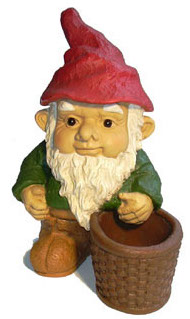
\includegraphics[width=60pt]{figures/chapter4/gnome.jpeg}};

%Shape: Rectangle [id:dp721778058251819] 
\draw  [line width=1.2]  (120,0) -- (320,0) -- (320,250) -- (120,250) -- cycle ;
%Right Arrow [id:dp5887472607772757] 
\draw  [line width=1.2]  (0,60) -- (75.25,60) -- (75.25,45) -- (100,75) -- (75.25,105) -- (75.25,90) -- (0,90) -- cycle ;
%Straight Lines [id:da03851464693257456] 
\draw    (180,50) -- (300,50) ;
%Straight Lines [id:da49911218049186523] 
\draw    (240,30) -- (240,130) ;
%Right Arrow [id:dp9356939686312407] 
\draw  [line width=1.2]  (100,200) -- (25,200) -- (25,215) -- (0,185) -- (25,155) -- (25,170) -- (100,170) -- cycle ;

% Text Node
\draw (210,40) node    {$x$};
% Text Node
\draw (270,40) node    {$f(x)$};
% Text Node
\draw (210,60) node    {\texttt{00101}};
% Text Node
\draw (210,80) node    {\texttt{11111}};
% Text Node
\draw (210,100) node    {\texttt{10111}};
% Text Node
\draw (210,120) node    {\texttt{00011}};
% Text Node
\draw (270,60) node    {\texttt{10101}};
% Text Node
\draw (270,80) node    {\texttt{01110}};
% Text Node
\draw (270,100) node    {\texttt{01011}};
% Text Node
\draw (270,120) node    {\texttt{10001}};
% Text Node
\draw (50,75) node    {$x$};
% Text Node
\draw (50,185) node    {$f( x)$};



\end{tikzpicture}
  \caption{一个忠实的侏儒实现了随机置换$f$}
  \label{fig:4-3}
\end{figure}

\subsection{强安全的分组密码}\label{subsec:4-1-3}

请注意,在攻击游戏 \ref{game:4-1} 中,解密算法 $D$ 从未被使用过。事实上,我们可以定义一个攻击游戏来给出一个更强的安全概念,在这个游戏中,对手被允许向挑战者发起两种类型的查询:
\begin{itemize}
	\item \textbf{前向查询}:对手向挑战者发送一个值 $x_i\in\mathcal{X}$,挑战者以 $y_i:=f(x_i)$ 应答对手;
	\item \textbf{反向查询}:对手向挑战者发送一个值 $y_i\in\mathcal{X}$,挑战者以 $x_i:=f^{-1}(y_i)$ 应答对手(在攻击游戏的实验$0$中,这是使用算法$D$完成的)。
\end{itemize}
接下来,我们可以为这个攻击游戏定义一个相应的优势。如果对于所有有效对手,这个优势都是可忽略不计的,我们就称这个分组密码是\textbf{强安全(strongly secure)}的。我们把这个定义的细节留给读者去解决(见练习 \ref{exer:4-9})。除了在后续章节中的一个应用实例(练习 \ref{exer:9-12})之外,我们不会在本文中使用这个概念。

\subsection{直接使用分组密码进行加密}\label{subsec:4-1-4}

既然分组密码是一种特殊的密码,我们当然可以考虑直接使用它进行加密。问题是,一个安全的分组密码是否也是语义安全的?

只要消息空间和数据分组空间相等,上面的问题的答案就是``是的"。下面的定理 \ref{theo:4-1} 将会指出这一点。然而在实践中,分组密码的数据分组非常短,正如我们之前提到的,AES 的数据分组只有 128 比特。如果我们想加密更长的消息,一个自然的想法是将一个长消息分解成一连串的数据分组,并对每个数据分组单独进行加密。这种使用分组密码来加密长消息的方法被称为\textbf{电子密码本模式 (electronic codebook mode, ECB)}。

更确切地说,假设 $\mathcal{E}=(E,D)$ 是一个定义在 $(\mathcal{K},\mathcal{X})$ 上的分组密码。对于任意多项式边界的 $\ell\geq1$,我们可以定义一个 $(\mathcal{K},\mathcal{X}^{\leq\ell},\mathcal{X}^{\leq\ell})$ 上的密码 $\mathcal{E}'=(E',D')$ 如下:
\begin{itemize}
	\item 对于 $k\in\mathcal{K}$ 和 $m\in\mathcal{X}^{\leq\ell}$,如果记 $v:=|m|$,我们定义:
	\[
    E'(k,m)=(E(k,m[0]),\dots,E(k,m[v-1]))
    \]
	\item 对于 $k\in\mathcal{K}$ 和 $c\in\mathcal{X}^{\leq\ell}$,如果记 $v:=|c|$,我们定义:
	\[
	D'(k,c)=(D(k,c[0]),\dots,D(k,c[v-1]))
	\]
\end{itemize}
图 \ref{fig:4-4} 展示了加解密的工作逻辑。我们称 $\mathcal{E}'$ 为\textbf{由 $\mathcal{E}$ 派生的 $\ell$ 次 ECB 密码 ($\ell$-wise ECB cipher derived from $\mathcal{E}$)}。

\begin{figure}
  \centering
  \subfigure[加密]{\tikzset{every picture/.style={line width=0.75pt}}

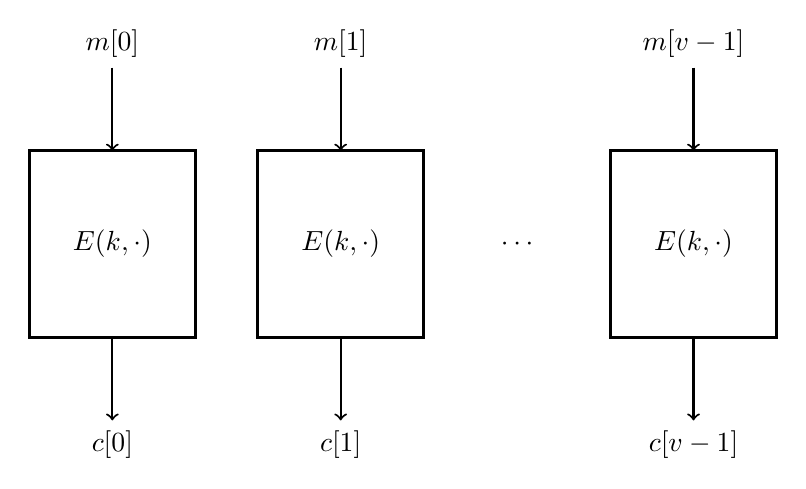
\begin{tikzpicture}[x=0.75pt,y=0.75pt,yscale=-1,xscale=1]

\draw  [line width=1.2]  (0,80) -- (80,80) -- (80,170) -- (0,170) -- cycle ;
\draw  [line width=1.2]  (110,80) -- (190,80) -- (190,170) -- (110,170) -- cycle ;
\draw  [line width=1.2]  (280,80) -- (360,80) -- (360,170) -- (280,170) -- cycle ;

\draw  [->]  (40,40) -- (40,80) ;
\draw  [->]  (40,170) -- (40,210) ;
\draw  [->]  (150,40) -- (150,80) ;
\draw  [->]  (150,170) -- (150,210) ;
\draw  [->]  (320,40) -- (320,80) ;
\draw  [->]  (320,170) -- (320,210) ;

\draw (40,125) node    {$E( k,\cdot )$};
\draw (40,36.6) node [anchor=south] [inner sep=0.75pt]    {$m[ 0]$};
\draw (40,213.4) node [anchor=north] [inner sep=0.75pt]    {$c[ 0]$};
\draw (150,125) node    {$E( k,\cdot )$};
\draw (150,36.6) node [anchor=south] [inner sep=0.75pt]    {$m[ 1]$};
\draw (150,213.4) node [anchor=north] [inner sep=0.75pt]    {$c[ 1]$};
\draw (320,125) node    {$E( k,\cdot )$};
\draw (320,36.6) node [anchor=south] [inner sep=0.75pt]    {$m[ v-1]$};
\draw (320,213.4) node [anchor=north] [inner sep=0.75pt]    {$c[ v-1]$};
\draw (235,125) node    {$\cdots $};


\end{tikzpicture}}
  
  \,
  
  \,
  
  \subfigure[解密]{\tikzset{every picture/.style={line width=0.75pt}}      

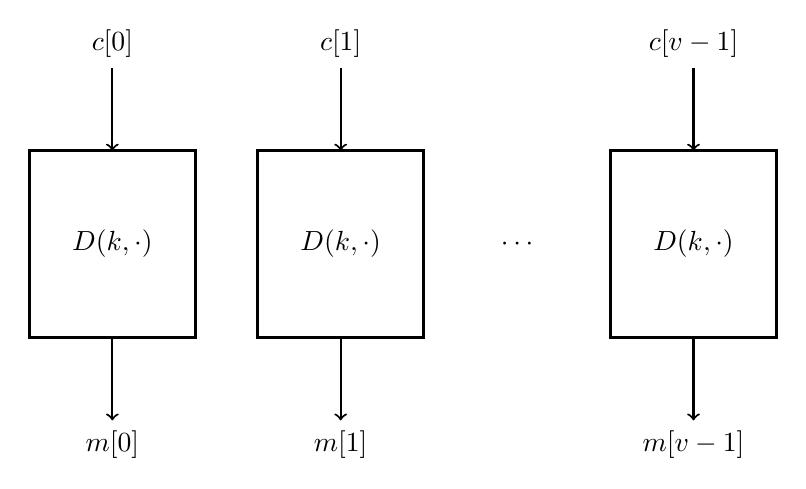
\begin{tikzpicture}[x=0.75pt,y=0.75pt,yscale=-1,xscale=1]


\draw  [line width=1.2]  (0,80) -- (80,80) -- (80,170) -- (0,170) -- cycle ;
\draw  [line width=1.2]  (110,80) -- (190,80) -- (190,170) -- (110,170) -- cycle ;
\draw  [line width=1.2]  (280,80) -- (360,80) -- (360,170) -- (280,170) -- cycle ;

\draw  [->]  (40,40) -- (40,80) ;
\draw  [->]  (40,170) -- (40,210) ;
\draw  [->]  (150,40) -- (150,80) ;
\draw  [->]  (150,170) -- (150,210) ;
\draw  [->]  (320,40) -- (320,80) ;
\draw  [->]  (320,170) -- (320,210) ;

\draw (40,125) node    {$D( k,\cdot )$};
\draw (40,36.6) node [anchor=south] [inner sep=0.75pt]    {$c[ 0]$};
\draw (40,213.4) node [anchor=north] [inner sep=0.75pt]    {$m[ 0]$};
\draw (150,125) node    {$D( k,\cdot )$};
\draw (150,36.6) node [anchor=south] [inner sep=0.75pt]    {$c[ 1]$};
\draw (150,213.4) node [anchor=north] [inner sep=0.75pt]    {$m[ 1]$};
\draw (320,125) node    {$D( k,\cdot )$};
\draw (320,36.6) node [anchor=south] [inner sep=0.75pt]    {$c[ v-1]$};
\draw (320,213.4) node [anchor=north] [inner sep=0.75pt]    {$m[ v-1]$};
\draw (235,125) node    {$\cdots $};


\end{tikzpicture}}
  \caption{ECB模式的加密与解密}
  \label{fig:4-4}
\end{figure}

ECB 密码与例 \ref{exmp:2-3} 和例 \ref{exmp:2-6} 中讨论的置换密码有非常密切的关系。主要区别在于,我们现在不是从 $\mathcal{X}$ 上所有可能的置换中完全随机地选择一个,而是在小得多的置换 $\{E(k,\cdot):k\in\mathcal{K}\}$ 中选择。另一个不太重要的区别是,在例 \ref{exmp:2-3} 中,我们定义的置换密码拥有定长的消息空间(这实际上只是一个任意的选择,因为我们也可以将置换密码定义在变长的消息空间上),而 ECB 密码的消息空间可以是变长的。除此以外,在例 \ref{exmp:2-3} 中,我们举了一个大小为 $27$ 的置换密码的例子,但如果我们使用像 AES 这样的分组长度为 $128$ 比特的密码,其``字母表"要大得多得多,事实上有 $2^{128}$ 那么大。尽管存在如此多的差异,例 \ref{exmp:2-6} 中讨论的置换密码的一些缺陷在 ECB 密码中也同样存在。下面我们举个例子。如果对两条消息 $m_0,m_1\in\mathcal{M}^2$ 进行 ECB 加密,其中 $m_0$ 由两个相同的分组组成(即 $m_0[0]=m_0[1]$),而 $m_1$ 由两个不同的分组组成(即 $m_1[0]\neq m_1[1]$),那么对手很容易就能区分出这两条消息的加密结果。单只因为这个原因,\emph{ECB 密码就不符合我们对语义安全的定义,因此,我们强烈反对将它作为加密方案使用}。

图 \ref{fig:4-5} 以图像的方式表现了这种能够轻易分辨相同明文分组的能力。这里,图像数据使用 ECB 模式加密,每个数据分组都来自对明文中小像素点的编码。由于相同的像素块会被映射到相同的密文上,所以原始图片中相同的像素在密文中也是相同的,我们可以从密文中依稀看到明文的轮廓。

但是请注意,也有一些例 \ref{exmp:2-6} 中讨论的缺陷在这里并不直接适用。假设我们在加密一个 ASCII 编码的文本。如果分组大小是 $128$ 比特,那么每个字符通常会被编码为一个字节,这样一个分组就由 $16$ 个字符组成。这时对手就无法像例 \ref{exmp:2-6} 中那样轻易地找到个别重复字符的位置了。

\vspace{10pt}

在本节的最后,我们将要表明,如果消息空间被限制为\emph{各不相同的}数据分组的序列,那么 ECB 模式实际上是安全的。这对于单个分组加密的特殊情况也是适用的。例如,假设我们使用的是 AES,它有 $128$ 比特的数据分组。那么,我们可以从每个数据分组中分配出 $32$ 比特作为计数器,并将剩余的 $96$ 比特作为承载消息的比特。有了这样的策略,我们可以将任何长达 $2^{32}\cdot 96$ 比特的消息编码为一串各不相同的数据分组。当然,这种策略的缺点是密文会比明文长 $33\%$。

\begin{figure}
  \centering
  \subfigure[明文]{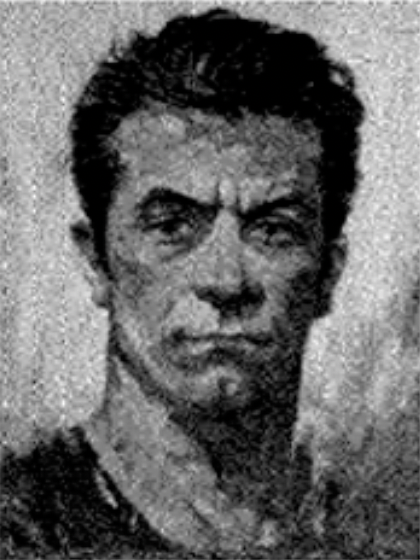
\includegraphics[width=0.21\linewidth]{figures/chapter4/fig5-a.png}}
  \quad\quad\quad\quad\quad
  \subfigure[使用AES在ECB模式下加密明文]{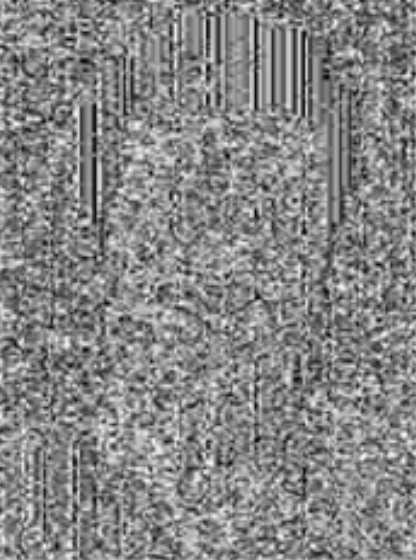
\includegraphics[width=0.21\linewidth]{figures/chapter4/fig5-b.png}}
  \caption{ECB模式中的加密}
  \label{fig:4-5}
\end{figure}

\begin{theorem}\label{theo:4-1}
令 $\mathcal{E}=(E,D)$ 是一个分组密码,$\ell\geq1$ 是任意多项式边界的值,令 $\mathcal{E}'=(E',D')$ 是由 $\mathcal{E}$ 派生的 $\ell$ 次 ECB 密码,但其消息空间被限制为最多 $\ell$ 个各不相同的数据分组的所有可能序列。如果 $\mathcal{E}$ 是一个安全的分组密码,那么 $\mathcal{E}'$ 就是一个语义安全的密码。
\begin{quote}
特别地,对于每个就 $\mathcal{E}'$ 进行攻击游戏 \ref{game:2-1} 的 SS 对手 $\mathcal{A}$,都存在一个就 $\mathcal{E}$ 进行攻击游戏 \ref{game:4-1} 的 BC 对手 $\mathcal{B}$,其中 $\mathcal{B}$ 是一个围绕 $\mathcal{A}$ 的基本包装器,满足:
\end{quote}
\begin{equation}\label{eq:4-3}
{\rm SS\mathsf{adv}}[\mathcal{A},\mathcal{E}']=2\cdot{\rm BC\mathsf{adv}}[\mathcal{B},\mathcal{E}]
\end{equation}
\end{theorem}

\begin{proof}[证明思路]
基本思想是,如果对手被赋予了一条消息的加密,而该消息是一串各不相同的数据分组,那么对手能看到的实际上也只是一个随机数据分组的序列(无替换采样)。
\end{proof}

\begin{proof}
如果 $\mathcal{E}$ 定义在 $(\mathcal{K},\mathcal{X})$ 上,令 $\mathcal{X}_*^{\leq\ell}$ 表示 $\mathcal{X}$ 中由最多 $\ell$ 个不同元素所组成的所有序列的集合。

令 $\mathcal{A}$ 是一个有效对手,它像攻击游戏 \ref{game:2-1} 中那样攻击 $\mathcal{E}'$。我们的目标是,假设 $\mathcal{E}$ 是一个安全的分组密码,证明 ${\rm SS\mathsf{adv}}[\mathcal{A},\mathcal{E}']$ 是可忽略不计的。使用语义安全攻击游戏的比特猜测版本更加方便。我们试图证明:
\begin{equation}\label{eq:4-4}
{\rm SS\mathsf{adv}}^*[\mathcal{A},\mathcal{E}']={\rm BC\mathsf{adv}}[\mathcal{B},\mathcal{E}]
\end{equation}
对于某个有效对手 $\mathcal{B}$ 成立。那么根据定理 \ref{theo:2-10},我们就能得到式 \ref{eq:4-3}。

所以,考虑对手 $\mathcal{A}$ 在攻击游戏 \ref{game:2-1} 的比特猜测版本中对 $\mathcal{E}'$ 的攻击。在这个游戏中,$\mathcal{A}$ 向挑战者发送两条长度相同的消息 $m_0,m_1$,然后挑战者选择一个随机密钥 $k$ 和一个随机比特 $b$,并用 $k$ 加密 $m_b$,将得到的密文 $c$ 交给 $\mathcal{A}$;最后,$\mathcal{A}$ 输出一个比特 $\hat b$。如果 $\hat b=b$,则对手 $\mathcal{A}$ 赢得游戏。

挑战者在该游戏中的逻辑可以表示如下:

\vspace*{10pt}

\hspace*{5pt} 当从对手 $\mathcal{A}$ 处收到消息 $m_0,m_1\in\mathcal{X}_*^{\leq\ell}$ 时,记 $v:=|m_0|=|m_1|$:\\
\hspace*{50pt} 选取 $b\overset{\rm R}\leftarrow\{0,1\}$\\
\hspace*{50pt} 选取 $k\overset{\rm R}\leftarrow\mathcal{K}$\\
\hspace*{50pt} 令 $c\leftarrow(E(k,m_b[0]),\dots,E(k, m_b[v-1]))$\\
\hspace*{50pt} 将 $c$ 发送给 $\mathcal{A}$。

\vspace*{10pt}

我们将该游戏称作\textbf{游戏 $\mathbf{0}$}。我们下面还将定义游戏 $1$ 和游戏 $2$。对于 $j=0,1,2$,我们定义 $W_j$ 为 $\mathcal{A}$ 在游戏 $j$ 中输出的 $\hat b=b$ 的事件。根据定义,我们有:
\begin{equation}\label{eq:4-5}
\mathrm{SS}\mathsf{adv}^*[\mathcal{A},\mathcal{E}']
=
|\Pr[W_0]-{1}/{2}|
\end{equation}

\noindent
\textbf{游戏 $\mathbf{1}$}。该游戏与游戏 $0$ 基本相同,只是现在,挑战者用一个随机的 $f\in{\rm Perms}[\mathcal{X}]$ 代替 $E(k,\cdot)$。我们的挑战者现在看起来是这样的:

\vspace*{10pt}

\hspace*{5pt} 当从对手 $\mathcal{A}$ 处收到消息 $m_0,m_1\in\mathcal{X}_*^{\leq\ell}$ 时,记 $v:=|m_0|=|m_1|$:\\
\hspace*{50pt} 选取 $b\overset{\rm R}\leftarrow\{0,1\}$\\
\hspace*{50pt} 选取 $f\overset{\rm R}\leftarrow{\rm Perms}[\mathcal{X}]$\\
\hspace*{50pt} 令 $c\leftarrow(f(m_b[0]),\dots,f(m_b[v-1]))$\\
\hspace*{50pt} 将 $c$ 发送给 $\mathcal{A}$。

\vspace*{10pt}

直观地说,$\mathcal{E}$ 是一个安全的分组密码的事实意味着,对手应该注意不到这个变化。为了严格地证明这一点,我们下面展示,如何构建一个分组密码对手 $\mathcal{B}$,使得它是一个围绕 $\mathcal{A}$ 的基本包装器,且满足:
\begin{equation}\label{eq:4-6}
\big\lvert
\Pr[W_0]-\Pr[W_1]
\big\rvert
=\mathrm{BC}\mathsf{adv}[\mathcal{B},\mathcal{E}]
\end{equation}

$\mathcal{B}$ 的设计直接来自于游戏 $0$ 和 $1$ 的逻辑。对手 $\mathcal{B}$ 就 $\mathcal{E}$ 进行攻击游戏 \ref{game:4-1},其工作原理如下:
\begin{quote}
记 $f$ 为 $\mathcal{B}$ 的分组密码挑战者在攻击游戏 \ref{game:4-1} 中选择的函数。我们让 $\mathcal{B}$ 扮演 $\mathcal{A}$ 的挑战者的角色,其工作逻辑如下:

\vspace*{5pt}

\hspace*{20pt} 当从对手 $\mathcal{A}$ 处收到消息 $m_0,m_1\in\mathcal{X}_*^{\leq\ell}$ 时,记 $v:=|m_0|=|m_1|$:\\
\hspace*{50pt} 选取 $b\overset{\rm R}\leftarrow\{0,1\}$\\
\hspace*{50pt} 令 $c\leftarrow(f(m_b[0]),\dots,f(m_b[v-1]))$\\
\hspace*{50pt} 将 $c$ 发送给 $\mathcal{A}$。

\vspace*{5pt}

请注意,$\mathcal{B}$ 通过查询它自己的分组密码挑战者来计算 $f(m_b[0]),\dots,f(m_b[v-1])$。最后,当 $\mathcal{A}$ 输出一个比特 $\hat b$ 时,$\mathcal{B}$ 输出 $\delta(\hat b,b)$,其中 $\delta$ 的定义见式 \ref{eq:3-7}。
\end{quote}

\vspace{8pt}

\noindent
显然,当 $\mathcal{B}$ 处于其攻击游戏的实验 $0$ 时,它会以 $\Pr[W_0]$ 的概率输出 $1$。而当 $\mathcal{B}$ 处于其攻击游戏的实验 $1$ 时,它会以 $\Pr[W_1]$ 的概率输出 $1$。这样,我们就能得到式 \ref{eq:4-6}。

\vspace{8pt}

\noindent
\textbf{游戏 $\mathbf{2}$}。
现在,我们重写游戏 $1$ 中的挑战者,让其使用我们在 \ref{subsec:4-1-2} 小节中讨论的``忠实的侏儒"来实现随机置换。$m_0$ 和 $m_1$ 的每条消息都需要由各不相同的数据分组组成(我们的挑战者不需要验证这一点),因此我们的侏儒的工作很容易:它甚至不需要看输入数据分组,因为这些数据分组被确保是各不相同的;然而,它仍然需要确保它产生的输出分组是各不相同的。

我们可以把我们的挑战者的逻辑表述如下:

\vspace*{10pt}

\hspace*{5pt} 选取 $y_0\overset{\rm R}\leftarrow\mathcal{X}$,$y_1\overset{\rm R}\leftarrow\mathcal{X}\setminus\{y_0\}$,$\dots$,$y_{\ell-1}\overset{\rm R}\leftarrow\mathcal{X}\setminus\{y_0,\dots,y_{\ell-2}\}$\\
\hspace*{26pt} 当从对手 $\mathcal{A}$ 处收到消息 $m_0,m_1\in\mathcal{X}_*^{\leq\ell}$ 时,记 $v:=|m_0|=|m_1|$:\\
\hspace*{50pt} 选取 $b\overset{\rm R}\leftarrow\{0,1\}$\\
\hspace*{50pt} 令 $c\leftarrow(y_0,\dots,y_{v-1})$\\
\hspace*{50pt} 将 $c$ 发送给 $\mathcal{A}$。

\vspace*{10pt}

由于我们的侏儒是忠实的,我们有:
\begin{equation}\label{eq:4-7}
\Pr[W_1]=\Pr[W_2]
\end{equation}
此外,我们声称:
\begin{equation}\label{eq:4-8}
\Pr[W_2]={1}/{2}
\end{equation}
这来自这样一个事实:在游戏 $2$ 中,对手的输出 $\hat b$ 是它自己的随机选择,以及 $y_0,\dots,y_{\ell-1}$ 的一个函数。由于这些值(根据定义)与 $b$ 无关,因此 $\hat b$ 和 $b$ 是相互独立的。所以式 \ref{eq:4-8} 成立。

综合式 \ref{eq:4-5},式 \ref{eq:4-6},式 \ref{eq:4-7} 和式 \ref{eq:4-8},我们就能得到式 \ref{eq:4-4},因此定理 \ref{theo:4-1} 得证。
\end{proof}

\subsection{数学细节}\label{subsec:4-1-5}

和之前一样,我们下面讨论一些之前被忽略了的数学细节。

由于分组密码只是一种特殊的密码,所以关于分组密码的定义,其实没有什么是 \ref{sec:2-3} 节中没有交代的。像往常一样,定义 \ref{def:4-1} 需要被正确地解释。首先,在攻击游戏 \ref{game:4-1} 中,我们要理解,对于安全参数 $\lambda$ 的每个值,我们都会得到一个不同的概率空间,它由挑战者的随机选择和对手的随机选择共同决定。其次,挑战者会产生一个系统参数 $\Lambda$,并在游戏一开始就将其发送给对手。第三,优势 ${\rm BC\mathsf{adv}}[\mathcal{B},\mathcal{E}]$ 是安全参数 $\lambda$ 的一个函数,安全性则意味着它是一个可忽略不计函数。